\section{Reflection security}\label{sec:refsec}

\subsection{The reflection game}\label{subsec:refsecgame}

Let $\mathcal{PE} = (Gen, \mathcal{E}, \mathcal{D})$ be a private-key encryption
scheme, $\mathcal{A}$ be an adversary and $\mathcal{S}$ be a simulator of
$\mathcal{A}$. The game
$\text{Game}_{\text{REF-SEC}}^{\mathcal{PE},\mathcal{A}}(\lambda,  f, g,
\mathcal{M})$ is parameterized with a rendering function $f(\cdot, \cdot,
\cdot)$, the security parameter $\lambda$, some function $g$ of the plaintext,
and a distribution of secrets $\mathcal{M}$ such that secrets $s$ that exist in
$\mathcal{M}$ it holds that $|s| = \lambda$. We require that the rendering
function $f$ is polynomially computable and reversible.

In the case of the example described above, the rendering function $f$ is the
rendering of the HTML response along with compression that is applied on it.
Function $g$ represents the prefix of the secret $s$ in the plaintext response.

The challenger produces a $\lambda$-bit key $k \leftarrow Gen(1^\lambda)$. The
challenger initially chooses a secret $s \leftarrow \mathcal{M}$. The adversary
is given $g$, $f$ and $\mathcal{M}$.

The adversary is then allowed to run and make arbitrary calls to a reflection
oracle. The oracle is parameterized by $s$, the secret unknown to the adversary.
For the reflection oracle call, the adversary chooses a reflection string $r$
and sends it to the oracle. The oracle computes $m = f(s, r)$. Subsequently $m$
is encrypted as $c = \mathcal{E}_\kappa(m)$, and $c$ is sent back to the
adversary.

In our previous example, the reflection oracle takes the form of the vulnerable
endpoint in the target service. This endpoint allows the adversary to issue an
arbitrary amount of requests containing a chosen parameter $r$ which is then
reflected in the plaintext response from the service, along with the secret $s$.
Since the adversary has network access via the sniffer component, he is able to
observe the response packets and collect the response ciphertext $c$.

When the adversary decides to complete the game, they output a guess $y$. The
adversary is successful if $g(s) = y$. In the case of Rupture, a successful
attack results in the decryption of a single character that extends the known
prefix of secret $s$.

Formally, let the public key adversarial game be defined as follows:

\begin{lstlisting}[texcl,mathescape,basicstyle=\small]
def $\text{Game}_{\text{REF-SEC}}^{\mathcal{PE},\mathcal{A}}(\lambda, f, \mathcal{M}, g)$:
    $k \leftarrow Gen(1^\lambda)$
    $s \leftarrow \mathcal{M}$
    $y \leftarrow \mathcal{A}^{\text{Reflect}^{\mathcal{E}_{k}}_s(r)}(\lambda, f, \mathcal{M}, g)$
    if $y = g(s)$:
        return 1
    else:
        return 0
\end{lstlisting}

Where the reflection oracle provided to the adversary is as follows:

\begin{lstlisting}[texcl,mathescape,basicstyle=\small]
def $\text{Reflect}^{\mathcal{E}_{k}}_s(r)$:
    $m = f(s, r)$
    $c \leftarrow \mathcal{E}_{k}(m)$
    return $c$
\end{lstlisting}

Let the simulator game be defined as follows:

\begin{lstlisting}[texcl,mathescape,basicstyle=\small]
def $\text{Game}_{\text{REF-SIM}}^{\mathcal{PE},\mathcal{S}}(\lambda, f, \mathcal{M}, g)$:
    $y \leftarrow \mathcal{S}(f, \mathcal{M}, g)$
    $s \leftarrow \mathcal{M}$
    if $y = g(s)$:
        return 1
    else:
        return 0
\end{lstlisting}

Where the simulator does not require an oracle for its execution.

The reflection game is depicted in Figure \ref{fig:refgame}.

    \begin{figure}[thpb]
        \centering
            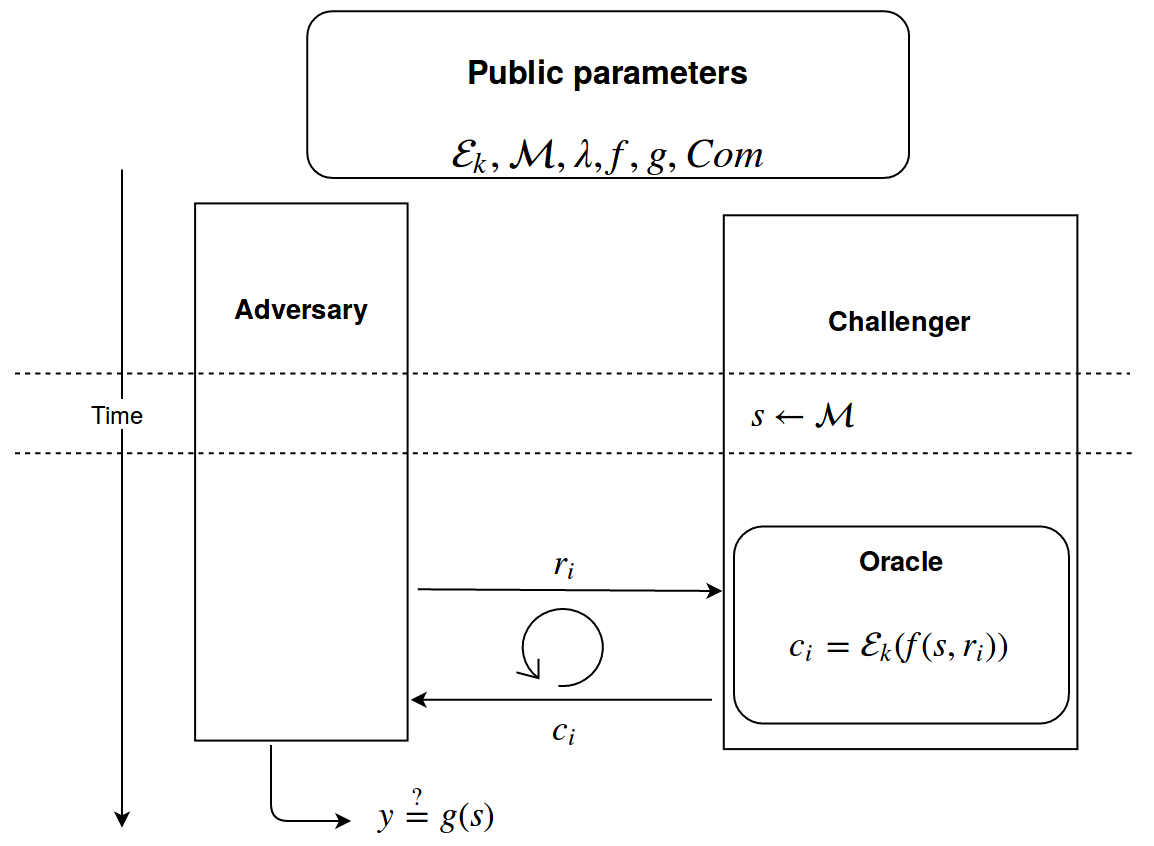
\includegraphics[width=0.48\textwidth]{figures/reflection_game.png}
        \caption{Reflection Game}
        \label{fig:refgame}
    \end{figure}

\subsection{Adversarial advantage}\label{subsec:refsecadv}

Let us now define the advantage of the adversary against a simulator:
\begin{align*}
    \text{Adv}_{\mathcal{PE}, \mathcal{A}, \mathcal{S}}&(\lambda, f, \mathcal{M}, g) &\defeq\\
    |\Pr[\text{Game}_{\text{REF-SEC}}^{\mathcal{PE},\mathcal{A}}(\lambda, f, \mathcal{M}, g) = 1] &-\\
    \Pr[\text{Game}_{\text{REF-SIM}}^{\mathcal{PE},\mathcal{S}}(\lambda, f, \mathcal{M}, g) = 1]| &
\end{align*}

\subsection{Adaptive reflection security}\label{subsec:adaptiverefsec}

Given a rendering function $f(\cdot, \cdot, \cdot)$, a public-key encryption
scheme $\mathcal{PE}$ is \textit{reflection-secure} if:
\begin{align*}
    \forall \mathcal{M}:
    \forall g:
    \forall PPT \mathcal{A}:
    \exists PPT \mathcal{S}:\\
    \text{Adv}_{\mathcal{PE}, \mathcal{A}, \mathcal{S}}(\lambda, f, \mathcal{M}, g) = negl(\lambda)
\end{align*}

\begin{lemma}[Semantic security]
    Let $(Gen, K, D)$ be a length-preserving reflection-secure encryption
    scheme. Then it is also semantically secure.
\end{lemma}

\begin{proof}
    We will prove that if the scheme is not semantically secure, then it is
    necessarily not reflection secure. Assume that the scheme is not
    semantically secure. Then there will exist a PPT adversary $\mathcal{A}$
    such that for all PPT simulators $\mathcal{S}$ we have that $\mathcal{A}$
    has non-negligible advantage to $\mathcal{S}$ in the semantic security game.

    We will now construct an adversary $\mathcal{A'}$ for the reflection
    security game. $\mathcal{A'}$ operates as follows: It makes one query to
    the reflection oracle setting $r_0 = \epsilon$ and receives a response $c_0
    = K_k(s, r_0) = K_k(s) = c$. It then passes that $c$ to the semantic
    security adversary $\mathcal{A}$. It answers all encryption and decryption
    queries of the semantic security adversary by relaying them to its own
    encryption and decryption oracle. Finally, when the semantic security
    adversary outputs $y = y'$, this $y'$ is output by the reflection security
    adversary. Note that $\mathcal{A}$ cannot distinguish whether they are
    playing against the actual semantic security game or being simulated by the
    reflection security adversary, as their view is identical. Therefore:

    \begin{equation}
        Pr[Game_{REF-SEC}^{\mathcal{A'}} = 1] = Pr[Game_{SEM-SEC}^{\mathcal{A}} = 1]
    \end{equation}

    It remains to prove that $\mathcal{A'}$ has significant advantage against
    any reflection simulator $\mathcal{S'}$. Indeed let $\mathcal{S'}$ be any
    reflection game simulator. We will construct a simulator $\mathcal{S}$ for
    the semantic security game. Initially, the simulator $\mathcal{S}$ receives
    the length of the ciphertext $|c|$. They then simulate the reflection game
    simulator $\mathcal{S'}$ as follows. Upon receiving query $r_i$ from the
    reflection game simulator, they answer with $|c| + |r_i|$. When the
    reflection security adversary outputs $y' = y$, this $y$ is output by the
    semantic security simulator. We observe that the reflection game simulator
    $\mathcal{S'}$ cannot distinguish whether they are playing against the
    actual simulated reflection game or being simulated by the semantic
    security simulator. To see this, note that from the length preservation
    assumption we have that $|c| + |r_i| = |K(s, r_i)| = |K(s', r_i)| =
    |K(0^{|s|}, r_i)|$. Therefore:

    \begin{equation}
        Pr[Game_{SEM-SIM}^{\mathcal{S}} = 1] = Pr[Game_{REF-SIM}^{\mathcal{S'}} = 1]
    \end{equation}

    From the assumption that the scheme is not semantically insecure, we know
    that:

    \begin{align*}
        |Pr[Game_{SEM-SEC}^{\mathcal{A}} = 1] - Pr[Game_{SEM-SIM}^{\mathcal{S}} = 1]| =\\
        Adv_{\mathcal{A}, \mathcal{S}} = \text{non-negl}
    \end{align*}

    And therefore, replacing both probabilities with their equals:

    \begin{align*}
        |Pr[Game_{REF-SEC}^{\mathcal{A'}} = 1] -
        Pr[Game_{REF-SIM}^{\mathcal{S'}} = 1]| =\\
        Adv_{\mathcal{A'}, \mathcal{S'}} = \text{non-negl}
    \end{align*}
\end{proof}
